% !TEX encoding = UTF-8 Unicode

%%
%% Copyright 2007, 2008, 2009 Elsevier Ltd
%%
%% This file is part of the 'Elsarticle Bundle'.
%% ---------------------------------------------
%%
%% It may be distributed under the conditions of the LaTeX Project Public
%% License, either version 1.2 of this license or (at your option) any
%% later version.  The latest version of this license is in
%%    http://www.latex-project.org/lppl.txt
%% and version 1.2 or later is part of all distributions of LaTeX
%% version 1999/12/01 or later.
%%
%% The list of all files belonging to the 'Elsarticle Bundle' is
%% given in the file `manifest.txt'.
%%
%% Template article for Elsevier's document class `elsarticle'
%% with numbered style bibliographic references
%% SP 2008/03/01
%%
%% $Id: elsarticle-template-num.tex 4 2009-10-24 08:22:58Z rishi $
%%
%% \documentclass[preprint,12pt,3p]{elsarticle}
%% \documentclass[preprint,review,12pt]{elsarticle}
%% \documentclass[final,1p,times]{elsarticle}
%% \documentclass[final,1p,times,twocolumn]{elsarticle}
%% \documentclass[final,3p,times]{elsarticle}
%% \documentclass[final,5p,times]{elsarticle}
%% \documentclass[final,5p,times,twocolumn]{elsarticle}

\documentclass[final,3p,times,twocolumn]{elsarticle}

% Packages
\usepackage{graphicx}
\usepackage[utf8]{inputenc}
\usepackage{textcomp,marvosym}
\usepackage{gensymb}
\usepackage{caption}
\usepackage{subcaption}
\usepackage[super]{nth}
\usepackage[inline]{enumitem}
\usepackage{moreenum}
\usepackage{tabulary}
\usepackage{tabu}
\usepackage{booktabs}
\usepackage{array}
\usepackage[super]{nth}
\usepackage{listings}
\usepackage{float}
\usepackage{upquote}
\usepackage{hyperref}
%\usepackage{minted}
%\usemintedstyle{bw}
\newcommand{\ra}[1]{\renewcommand{\arraystretch}{#1}}

% Special characters
\usepackage{gensymb}
\usepackage{amsmath,amssymb}
\usepackage{pifont}
\newcommand{\cmark}{\ding{51}}
\newcommand{\xmark}{\ding{55}}

\journal{Geomorphology}

\begin{document}

\begin{frontmatter}

\title{Dynamic Landscape Evolution}

\author[cga,la]{Brendan Harmon\corref{cor1}}
\cortext[cor1]{Corresponding author}
\ead{brendan.harmon@gmail.com}
%\ead[url]{baharmon@github.io}
%\ead[url]{https://github.com/baharmon/landscape_evolution}

\author[cga,meas]{Helena Mitasova}
\ead{hmitaso@ncsu.edu}

\author[cga,meas]{Vaclav Petras}
\ead{vpetras@ncsu.edu}

\author[cga,meas]{Anna Petrasova}
\ead{akratoc@ncsu.edu}

\address[cga]{Center for Geospatial Analytics, North Carolina State University, Raleigh, North Carolina, United States of America}
\address[la]{Robert Reich School of Landscape Architecture, Louisiana State University, Baton Rouge, Louisiana}
\address[meas]{Department of Marine, Earth, and Atmospheric Sciences, North Carolina State University, Raleigh, North Carolina, United States of America}

\begin{abstract}
While there are numerical landscape evolution models
that simulate how steady state flows of water and sediment
reshape topography over long periods of time, 
this is the first to simulate topographic change 
based on dynamic flows. 
It is a process-based, spatially distributed model
that uses the water and sediment flow continuity equations
to simulate how overland sediment mass flows 
reshape topography. 
This either steady state or dynamic model can simulate 
how topography will evolve for a range of hydrologic soil erosion regimes
based on topographic, land cover, soil, and rainfall parameters. 
A case study demonstrates how the behavior and results of 
the dynamic model differ the steady state model. 
The dynamic model is more accurate and 
demonstrates cross-scale interactions between 
topographic form and sediment flow processes.
%This is a fine-scale, short term, process-based landscape evolution model 
%using simulated erosion and deposition 
%to generate a time-series of digital elevation models 
%and compute the net change in elevation. 
%This model uses a path sampling method 
%to solve water and sediment flow continuity equations and 
%model mass flows over complex topographies 
%based on topographic, land cover, soil, and rainfall parameters. 
%This either steady state or dynamic model can simulate landscape evolution 
%for a range of hydrologic soil erosion regimes. 
%
%This process-based, spatially distributed landscape evolution model 
%simulates mass flows over complex topographies 
%based on topographic, land cover, soil, and rainfall parameters. 
%It can simulate landscape evolution for different soil erosion regimes 
%across a wide range of spatiotemporal scales 
%using either the simulated water erosion (SIMWE) model, 
%the unit stream power erosion deposition (USPED) model, 
%or the 3-dimensional revised universal soil loss equation (RUSLE 3D) model. 
%SIMWE is a physics-based simulation of water flow and erosion-deposition 
%based on the continuity equations (Mitasova et al. 2004). 
%This model has been implemented as an add-on module 
%for a free, open-source geographic information system – GRASS GIS.  
%It supports multithreading and parallel processing for the efficient computation 
%of physics-based simulations with large, high resolution topographic datasets. 
\end{abstract}

\begin{keyword}
%% keywords here, in the form: keyword \sep keyword
landscape evolution \sep dynamic model \sep continuity equations
%% MSC codes here, in the form: \MSC code \sep code
%% or \MSC[2008] code \sep code (2000 is the default)
\end{keyword}
%
\end{frontmatter}

% -------------- TOC --------------
\tableofcontents
\vfil
\pagebreak

% -------------- BODY --------------

\section{Introduction}

Landscape evolution models represent how the surface of the earth changes over time. 
Most studies of landscape evolution have been descriptive and qualitative, 
but a number of quantitative, numerical landscape evolution models 
have been developed 
that simulate elevational change over time 
\cite{Temme2013}. 
Numerical landscape evolution models
such as the Channel-Hillslope Integrated Landscape Development (CHILD) model 
\cite{Tucker2001} 
% CAESAR
and SIBERIA \cite{Willgoose2005} 
simulate steady state flows over long temporal scales. 
There are still, however, major research questions 
to address in the theoretical foundations of erosion modeling 
such as how erosional processes scale over time and space 
and how sediment detachment and transport interact \cite{Mitasova2013}. 
A dynamic landscape evolution model is needed to study 
fine-scale spatial and short-term temporal erosional processes
such as gully formation. %and morphodynamics.

% high resolution topographic data increasingly available from lidar and uav stereophotogrammetry
% value of fine scale model 

The dynamic landscape evolution model
is a process-based, spatially distributed model
that solves the water and sediment flow equations 
with Monte Carlo path sampling method
\cite{Mitasova2004}
to model mass flows over complex topographies 
based on topographic, land cover, soil, and rainfall parameters.
The modeled flow of sediment -- 
a function of water flow and soil detachment and transport parameters -- 
is then used to estimate the net erosion and deposition rates 
and the associated short-term evolution of the topography. 
During a simulation the model can switch between 
dynamic and steady state flow regimes. 

The dynamic landscape evolution model
has been implemented as the add-on module 
\textit{r.evolution}
\footnote{\url{https://github.com/baharmon/landscape\_evolution}} 
% also cite software release doi
for the free, open source
Geographic Resources Analysis Support System (GRASS) GIS.
%
This highly adaptable
geographic information system (GIS)-based implementation
can simulate landscape evolution 
for different soil erosion regimes
across a range of spatiotemporal scales
using either
the Simulated Water Erosion (SIMWE) model, 
the Unit Stream Power Erosion Deposition (USPED) model,
or the 3-dimensional Revised Universal Soil Loss Equation (RUSLE 3D) model.  
%
It supports multithreading and parallel processing
to efficiently compute simulations 
using large, high resolution topographic datasets.
%
It was developed as a tool to study 
the interaction of sediment detachment and transport
and the scaling erosional processes over time and space. 

%% TESTING & VALIDATION
%The model has been tested and validated
%using high resolution lidar time series. 

%a series of tests comparing simulated landscape evolution against recorded elevation change for a highly eroded watershed with active gully formation in Fort Bragg, North Carolina. These  tests will compare the performance of the different erosion models – SIMWE, USPED, and RULSE3D – and dynamic versus steady state models. In 2017 I compiled a geospatial dataset with a time series of high-resolution, lidar-based digital elevation models and a time series landcover based on automatically classified orthoimagery and lidar. Using the lidar time series I computed elevation change at 30 cm resolution to use for validation. 

%% 
%% RESULTS
%
%The tests show that % for ...
%gullies
%dynamic behavior at the beginning of a rain event
%before
%achieving steady state
%has a 
%
%development of
%creating microtopography
%such as ridges beside the gully channel
%
%% APPLICATIONS
%Applications include
%testing theories, 
%designing erosion control measures,
%developing scenarios for land planning and management
%etc

%
\subsection{Theory}

%Steady state versus dynamic flows \\
%
%Soil erosion regimes \\
%
%
%% DETACHMENT LIMITED  - RUSLE
%%
%%Both USLE and RUSLE consider erosion only along the flow line
%%without the influence of flow convergenceJdivergence 
%%and the equations can be properly applied only to areas experiencing net erosion. 
%%Depositional areas should be excluded.
%%Both the standard and modified equations can be properly applied only to areas experiencing net erosion. 
%%Depositional areas should be excluded from the study area 
%%because the model assumes that transport capacity exceeds detachment capacity everywhere 
%%and erosion and sediment transport is detachment capacity limited. 
%%Therefore, direct application of USLE/RUSLE to complex terrain within GIS is rather restricted. 
%%The results can also be interpreted as an extreme case with maximum possible spatial extent of erosion.


%Spatial and temporal scales \\

%% RUSLE3D 
%% useful for large datasets (up to 2 billion cells)
%% scale (see Panama and Yakima, see Panagos on r-factor)

%Erosion models \\

%Erosion to landscape evolution \\

%Dynamic evolution \\



\subsection{Aims and objectives}
% Testing and case studies
% Research aims and objectives

\subsection{Conceptual model}

%Diagram\\

%Dynamic vs steady state \\

%Determine mode \\
%Run erosion model \\
%Gravitational diffusion \\


% table of erosion models
\begin{table*}
\small
\caption{GIS-based soil erosion models}
\begin{tabu} to \textwidth {XXXXXl}
\toprule
Model & Spatial scale &  Temporal scale & Representation & GIS & Reference\\
\midrule
%
%USLE & landscape & annual & raster & map algebra & \cite{Wischmeier1978}\\
RUSLE3D & landscape & annual & raster & map algebra & \cite{Mitasova1996}\\ % annual -- event?
USPED & watershed & annual & raster & map algebra & \cite{Mitasova1996}\\ %annual -- event?
SIMWE & watershed & annual -- event & raster & module & \cite{Mitas1998}\\
%
\bottomrule
\\
\multicolumn{6}{c}{Adapted from Mitasova et al. \cite{Mitasova2013}}
\end{tabu}
\label{table:evolution_models} 
\end{table*}

% table of landscape evolution models
\begin{table*}
\small
\caption{Numerical landscape evolution models}
\begin{tabu} to \textwidth {XXXXXXl}
\toprule
Model & Spatial scale &  Temporal scale & Representation & Dynamics & GIS & Reference\\
\midrule
%
SIBERIA & landscape & continuous & raster & steady state & & \cite{Willgoose2005}\\
CHILD & landscape & continuous & mesh & steady state & & \cite{Tucker2001}\\
r.landscape.evol  & landscape & continuous & raster &  steady state & module & \cite{Barton2010}\\ 
r.evolution & watershed -- & event -- & raster & dynamic -- & module &\\ %cite software
& landscape & continuous && steady state & &\\
%
\bottomrule
\\
\multicolumn{7}{c}{Adapted from Mitasova et al. \cite{Mitasova2013}}
\end{tabu}
\label{table:evolution_models} 
\end{table*}

% r.land.evol uses r.watershed and RUSLE

\clearpage

% --------------------------------EROSION-DEPOSITION --------------------------------
\section{Simulation of water erosion model} \label{simwel}

SIMWE -- the Simulation of Water Erosion model -- 
is a physics-based simulation of shallow overland water and sediment flow
that uses a path sampling method to solve the continuity and momentum equations 
with a 2D diffusive wave approximation 
\cite{Mitas1998,Mitasova2001,Mitasova2004}.
%
It has been implemented in GRASS GIS as the modules 
r.sim.water\footnote{\url{https://grass.osgeo.org/grass75/manuals/r.sim.water.html}} 
and r.sim.sediment \footnote{\url{https://grass.osgeo.org/grass75/manuals/r.sim.sediment.html}}.

% overview
In SIMWE mode 
for each time step
the dynamic landscape evolution model 
determines the soil erosion regime,
simulates water and sediment flows, 
and then evolves the topography. 
% erdep
In an erosion-deposition regime 
the model 
computes the partial derivatives of the topography,
simulates shallow water flow and erosion-deposition,
and then evolves the topography based on the erosion-deposition rate
and gravitational diffusion.
% transport limited
The same process is used in
a transport capacity limited regime
except that the topography is evolved based on 
the transport limited erosion-deposition rate
and gravitational diffusion.
% detachment  limited
In a detachment capacity limited regime
the model instead
computes the partial derivatives of the topography,
simulates shallow water flow and sediment flow,
and then evolves the topography based on the sediment flow rate
and gravitational diffusion.

% dynamic versus steady state
The model simulates dynamic landscape evolution 
when the time step is less than the travel time 
for a drop of water or a particle of sediment to cross the landscape.
With longer time steps the model simulates steady state dynamics. 

\subsection{Erosion regime}
This model can switch erosion regimes at each time step
based on the rainfall intensity $i_r$
and the balance of the sediment detachment capacity $D_c$
and the sediment transport capacity $T_c$
represented by the first order reaction term $\sigma$ 
which depends on soil and landcover properties.
The detachment capacity is the maximum potential detachment rate by overland flow, while
the sediment transport capacity is the maximum potential sediment flow rate.
%Both are functions of shear stress.

% erosion regime eq.
\begin{equation}
\label{eq:regime}
\sigma = {D_c \over T_c}
\end{equation}
%
{\small
\noindent
where: \\
\noindent
\hspace*{0.5em} $\sigma$  is a first order reaction term ($m^{-1}$)\\
\hspace*{0.5em} $D_c$ is the sediment detachment capacity ($kg~m^{-1}s^{-1}$)\\
\hspace*{0.5em} $T_c$ is the sediment transport capacity ($kg~m^{-1}s^{-1}$)\\
}

%% erosion regime eq.
%\begin{equation}
%\label{eq:regime}
%\sigma({x,y})={D_c({x,y}) \over T_c({x,y})}
%\end{equation}
%
%{\small
%\noindent
%where: \\
%\noindent
%\hspace*{0.5em} $D_c({x,y})$ is the sediment detachment capacity ($kg~m^{-1}s^{-1}$)\\
%\hspace*{0.5em} $T_c({x,y})$ is the sediment transport capacity ($kg~m^{-1}s^{-1}$)\\
%\hspace*{0.5em} $\sigma({x,y})$  is a first order reaction term ($m^{-1}$) \\
%}

When rainfall intensity is very high ($i_r \geq 60 mm~hr^{-1}$)
or $\sigma$ is low ($\sigma \leq 0.01 m^{-1}$),
then the regime is detachment capacity limited. 
%
When rainfall intensity is not very high ($i_r < 60 mm~hr^{-1} $)
and $\sigma$ is high ($\sigma \geq 100 m^{-1}$),
then the regime is transport capacity limited. 
%
When rainfall intensity is not very high ($i_r<60 mm~hr^{-1}$)
and $\sigma$ is neither high nor low ($ 0.01 m^{-1}< \sigma < 100 m^{-1}$),
then there is an erosion-deposition regime. \\

\subsection{Shallow water flow}
The SIMWE model
simulates shallow overland water flow 
controlled by spatially variable topographic, soil, landcover, and rainfall parameters
by solving the continuity and momentum equations 
for steady state water flow with a path sampling method. 
Shallow water flow $q(x,y,t)$ can be approximated by
the bivariate form of the St.~Venant equation:

% shallow water flow eq.
\begin{equation}
\label{eq:water}
{\partial h(x,y,t) \over \partial t} =
 i_e(x,y,t) - \nabla ~ q(x,y,t)
\end{equation}
%
{\small
\noindent
where: \\
\noindent
\hspace*{0.5em} $(x,y)$ is the position ($m$)\\
\hspace*{0.5em} $t$ is the time ($s$) \\
\hspace*{0.5em} $h(x,y,t)$ is the depth of overland flow ($m$)\\
\hspace*{0.5em} $i_e(x,y,t)$ is the rainfall excess ($m~s^{-1}$) \\
\hspace*{0.5em} (i.e.~rainfall intensity $-$ infiltration $-$ vegetation intercept)\\
\hspace*{0.5em} $\nabla$ is the divergence of the flow vector field\\
\hspace*{0.5em} $q(x,y,t)$ is the water flow per unit width ($m^2~s^{-1}$). \\
}

Diffusive wave effects can be approximated
so that water can flow through depressions 
by integrating a diffusion term $ \propto \nabla^2 [h^{5/3}(x,y)]$ 
into the solution of the continuity and momentum equations 
for steady state water flow.
This equation is solved using a 
Green's function Monte Carlo path sampling method. 

%  diffuse wave eq.
\begin{equation}
\label{eq:difwater}
-{\varepsilon(x,y)\over 2 }\nabla^2 [h^{5/3}(x,y)]
+\nabla ~ [ h(x,y)~v(x,y)] = i_e(x,y)
\end{equation}
%
{\small
\noindent
 where: \\
 \noindent
 \hspace*{0.5em} $\varepsilon(x,y)$ is a spatially variable diffusion coefficient. \\
}

\subsection{Sediment flow}
In SIMWE the sediment flow rate $q_s(x,y,t)$ is estimated 
as a function of water flow and sediment concentration:

%sediment flow equation
\begin{equation}\label{eq:sedflow} 
q_s(x,y,t) = \rho_s(x,y,t) ~ q(x,y,t)
\end{equation}
%
{\small
\noindent
where: \\
\hspace*{0.5em} $q_s(x,y,t)$ is the sediment flow rate per unit width ($kg~m^{-1}s^{-1}$)\\
\hspace*{0.5em} $\rho_s(x,y,t)$ is sediment mass density ($kg~m^{-3}$).\\
%\hspace*{0.5em} $q(x,y,t)$ is unit flow discharge vector ($m^{2} s^{-1}$) \\
%\hspace*{0.5em} (i.e.~ the direction and rate of water flow per unit width)\\
}

\subsection{Erosion-deposition}
In SIMWE 
the net erosion-deposition rate is estimated
using the bivariate form of sediment continuity equation
to model sediment storage and flow 
based on effective sources and sinks.
Net erosion-deposition $d_s(x,y,t)$
-- the difference between sources and sinks --
is approximated by
the steady state sediment flow equation with diffusion:

% erosion-deposition equation
\begin{equation}\label{eq:sediment} 
d_s(x,y,t) = 
{\partial [\rho_sc(x,y,t)h(x,y,t)] \over \partial t} +
\nabla ~ q_s(x,y,t)
\end{equation}
%
{\small
\noindent
where: \\
\hspace*{0.5em} $d_s(x,y,t)$ is net erosion-deposition $(kg ~ m^{-2} s^{-1})$.\\
%\hspace*{0.5em} $q_s(x,y,t)$ is the sediment flow rate per unit width ($kg~m^{-1}s^{-1}$)\\
%\hspace*{0.5em} $\rho_s(x,y,t)$ is sediment mass density ($kg~m^{-3}$).\\
}

%\begin{equation}\label{eq:sediment} 
%D(x,y,t) = \mathrm{source - sinks} =
%{\partial [\rho_sc(x,y,t)h(x,y,t)] \over \partial t} +
%\nabla ~ q_s(x,y,t)
%\end{equation}

%Sources and sinks of sediment are assumed to be proportional to
%the difference between sediment transport capacity
%and the sediment flow rate: 
%\begin{equation}\label{eq:sources_sinks} 
%d_s = \sigma [T_c  - |q_s|]
%\end{equation}

% ADD transport limited erosion-deposition

\subsection{Landscape evolution}
The simulated change in elevation $\Delta z(x,y,t)$ due to water erosion and deposition
is a function of
the change in time, the net erosion-deposition rate, and the sediment mass density 
\cite{Mitasova2013}:

% landscape evolution equation
% change in elevation (m) = change in time (s) * net erosion-deposition (kg/m^2s) / sediment mass density (kg/m^3)
\begin{equation}
\label{eq:evolution} 
{\Delta z(x,y,t) = \Delta t ~ d_s(x,y,t) ~ \rho_s^{-1} }
\end{equation}

%{\small
%\noindent
%where: \\
%\noindent
%\hspace*{0.5em} $\Delta z =$ change in elevation $(m)$ \\
%\hspace*{0.5em} $d_s =$ net erosion-deposition $(kg ~ m^{-2} s^{-1})$ \\
%\hspace*{0.5em} $\rho_s c(x,y,t)$ = sediment mass density $(kg ~m^{-3})$\\ %[kg/m$^3$]
%\hspace*{0.5em} $\rho_s =$ sediment mass density $(kg ~m^{-3})$ \\
%}

% detachment limited landscape evolution
In a detachment limited erosion regime
the simulated change in elevation $\Delta z(x,y,t)$
is a function of
the change in time, the sediment flow rate, and the mass of water carried sediment per unit area
\cite{Mitasova2013}:

% change in elevation (m) = change in time (s) * sediment flux (kg/ms) / mass of sediment per unit area (kg/m^2)
\begin{equation}
\label{eq:flux_evolution} 
{\Delta z(x,y,t) = \Delta t ~ q_s(x,y,t) ~ \varrho_s^{-1} } 
\end{equation}
% \varrho_s(r)^{-1}
%
{\small
\noindent
where: \\
\noindent
%\hspace*{0.5em} $\Delta z =$ change in elevation $(m)$ \\
%\hspace*{0.5em} $q_s =$ sediment flux $(kg ~ m^{-1} s^{-1})$ \\
\hspace*{0.5em} $\varrho_s$ is the mass of sediment per unit area $(kg ~ m^{-2})$.\\
}

% gravitational diffusion
\noindent
Gravitational diffusion is then applied to the evolved topography
to simulate the settling of sediment particles. 
The simulated change in elevation $\Delta z(x,y,t) $ due to gravitational diffusion 
is a function of the change in time, the sediment mass density, 
the gravitational diffusion coefficient, and topographic divergence 
-- i.e.~the sum of the second order derivatives of elevation
\cite{thaxton2004}:

%gravitional diffusion eq.
% change in elevation (m) = elevation (m) - (change in time (s) / sediment mass density (kg/m^3) * gravitational diffusion coefficient (m^2/s) * divergence (m^-1))
\begin{equation}
\label{eq:grav_diffusion} 
{\Delta z(x,y,t) = \Delta t ~ \rho_s^{-1} ~ \varepsilon_g ~ \nabla(x,y,t)}
\end{equation}
%
{\small
\noindent
where: \\
\noindent
%\hspace*{0.5em} $\Delta z =$ change in elevation $(m)$ \\
%\hspace*{0.5em} $\rho_s c(x,y,t)$ = sediment mass density $(kg ~m^{-3})$\\ %[kg/m$^3$]
%\hspace*{0.5em} $\rho_s =$ sediment mass density $(kg ~m^{-3})$ \\
\hspace*{0.5em} $\varepsilon_g$ is the gravitational diffusion coefficient $(m^{2} s^{-1})$\\ %$(m^{-2} s^{-1})$
\hspace*{0.5em} $\nabla(x,y,t)$ is the topographic divergence $(m^{-1})$.\\
}

% -------------------------------- RUSLE --------------------------------
\section{Revised universal soil loss equation 3D model}
\label{rusle_model} % detachment limited
%RUSLE
The Revised Universal Soil Loss Equation for Complex Terrain (RUSLE3D) 
is an empirical equation for computing erosion 
in a detachment-capacity limited soil erosion regime
for watersheds with complex topography \cite{Mitasova1996}. 
% USLE
It is based on 
the Universal Soil Loss Equation (USLE),
an empirical equation for estimating the average
sheet and rill soil erosion from rainfall and runoff
on agricultural fields and rangelands with simple topography 
\cite{Wischmeier1978}. 
It models erosion dominated regimes without deposition
in which sediment transport capacity is uniformly greater than detachment capacity.
As an empirical equation the predicted soil loss 
is spatially and temporally averaged. 
In USLE soil loss per unit area is determined by 
an erosivity factor $R$,
a soil erodibility factor $K$, 
a slope length factor $L$,
a slope steepness factor $S$,
a cover management factor $C$,
and a prevention measures factor $P$.
These factors are empirical constants derived 
from an extensive collection of measurements 
%22.13m with 9\% slope
on 22.1m standard plots with an average slope of 0.09$\degree$.  
%
RUSLE3D was designed to account for more complex, 3D topography 
with converging and diverging flows. 
In RUSLE3D the topographic potential for erosion at any given point 
is represented by a 3D topographic factor $LS_{3D}$,
which is a function of the upslope contributing area %flow accumulation
and the angle of the slope. 

In this spatially and temporally distributed model 
RUSLE3D is modified by the use of a 
event-based r-factor derived from the rainfall intensity at each time step.
%
For each time step
this model computes the parameters for RUSLE3D -- 
an event-based erosivity factor,
the slope of the topography, the flow accumulation, and
the 3D topographic factor -- and then
solves the RUSLE3D equation for sediment flow. 
The sediment flow is used to simulate landscape evolution 
in a detachment capacity limited soil erosion regime.

% RESOURCES
% https://ncsu-geoforall-lab.github.io/erosion-modeling-tutorial/erdep_theory.html
% http://www4.ncsu.edu/~hmitaso/gmslab/reports/CerlErosionTutorial/denix/denixstart.html

\subsection{Event-based r-factor derivation} % (MJ mm ha^-1 hr^-1)
In USLE and RUSLE the erosivity factor $R$ is the 
combination of the total energy and peak intensity of a rainfall event,
representing the interaction between the detachment of sediment particles
and the transport capacity of the flow. 
It can be calculated as the product of the 
the kinetic energy of the rainfall event $E$
and its maximum 30-minute intensity $I_{30}$
\cite{Brown1987,Renard1997}.
%
In this model, however, the erosivity factor
is derived at each time step as a function of
kinetic energy, rainfall volume, rainfall intensity, and time.
%
First rain energy is derived from rainfall intensity \cite{Brown1987}:
% rain energy eq.
\begin{equation}
\label{eq:rain_energy}
{e_r = 0.29 ~ (1.-0.72 ~ exp(-0.05 ~ i_r))}
\end{equation}
%
{\small
\noindent
where: \\
\noindent
\hspace*{0.5em} $e_r$is unit rain energy $(MJ ~ ha^{-1} ~ mm{^-1})$\\
\hspace*{0.5em} $i_r$ is rainfall intensity $(mm ~ h^{-1})$.\\
}

\noindent
Then the event-based erosivity index $R_e$ is calculated as:
%the product of unit rain energy, rainfall volume, rainfall intensity, and time: 
% event erosivity index (MJ mm ha^-1 hr^-1)
\begin{equation}
\label{eq:erosivity_index}
{R_e = e_r ~ v_r ~ i_r ~ t_r}
\end{equation}
%
{\small
\noindent
\hspace*{0.5em} $R_e$ is the event-based erosivity index $(MJ ~ mm ~ ha^{-1} ~ hr^{-1})$\\
%\hspace*{0.5em} $e_r$ is unit rain energy $(MJ ~ ha^{-1} ~ mm{^-1})$\\
\hspace*{0.5em} $v_r$ is rainfall volume $(mm)$ derived from ${v_r = i_r ~ t_r}$\\
%\hspace*{0.5em} $i_r$ is rainfall intensity $(mm ~ h^{-1})$\\
\hspace*{0.5em} $t_r$ is time interval $s$\\ 
}
%derive event erosivity index (MJ mm ha^-1 hr^-1)
%then multiply by rainfall interval in seconds (MJ mm ha^-1 hr^-1 s^-1)

\subsection{Flow accumulation}
The upslope contributing area is determined by flow accumulation. 
Flow accumulation is calculated using a multiple flow direction algorithm \cite{Metz2009} 
based on $A^{T}$ least cost paths \cite{Ehlschlaeger1989}. 
The multiple flow direction algorithm 
implemented in GRASS GIS as the module 
\textit{r.watershed}\footnote{https://grass.osgeo.org/grass72/manuals/r.watershed.html}
is computationally efficient and can
navigate nested depressions and other obstacles. 


\subsection{3D topographic factor}
The 3D topographic factor $LS_{3D}(x,y)$
is calculated as a function of 
the flow accumulation,
representing the upslope contributing area,
and the slope. 
%
The empirical coefficients $m$ and $n$
for the upslope contributing area 
and the slope
can range from $0.2$ to $0.6$
and $1.0$ to $1.3$ respectively
with low values representing dominant sheet flow
and high values representing dominant rill flow.
%http://www4.ncsu.edu/~hmitaso/gmslab/papers/erijgis.html

%with the higher values reflecting the pattern for prevailing rill erosion with more turbulent flow when erosion sharply increases with the amount of water. Lower exponent values close to m = n = 1 better reflect the pattern of compounded, long term impact of both rill and sheet erosion and averaging over a long term sequence of large and small events.

\begin{equation}
\label{eq:ls_factor}
{LS_{3D}(x,y) = (m+1.0) ~ (a(x,y) ~ a_0^{-1})^{m} ~ (sin(\beta) / \beta_0)^{n}}
\end{equation}
%
{\small
\noindent
where: \\
\noindent
\hspace*{0.5em} $LS_{3D}$ is the dimensionless topographic (length-slope) factor\\
\hspace*{0.5em} $a$ is flow accumulation $(m)$\\
\hspace*{0.5em} $a_0$ is the length of the standard USLE plot $(22.1 m)$\\
\hspace*{0.5em} $\beta$ is the slope angle $(\degree)$\\
\hspace*{0.5em} $m$ is an empirical coefficient\\
\hspace*{0.5em} $n$ is an empirical coefficient\\
\hspace*{0.5em} $\beta_0$ is the slope of the standard USLE plot $(0.09 \degree)$\\
}

\subsection{Sediment flow} 
The sediment flow is a function of the event-based erosivity factor, 
the soil erodibility factor, the 3D topographic factor, cover factor, and the prevention measures factor:
%
\begin{equation}
\label{eq:rusle}
{E = R_e ~ K ~ LS_{3D} ~ C ~ P}
\end{equation}
%
{\small
\noindent
where: \\
\noindent
\hspace*{0.5em} $E$ is soil loss $(kg ~ m^{-2} ~ min^{-1})$\\
\hspace*{0.5em} $R_e$ is the event-based erosivity factor $(MJ ~ mm ~ ha^{-1} ~ hr^{-1})$\\ %~  s{^-1}
\hspace*{0.5em} $K$ is the soil erodibility factor $(ton ~ ha ~ hr ~ ha^{-1} ~ MJ^{-1} ~ mm^{-1})$\\
\hspace*{0.5em} $LS_{3D}$ is the dimensionless topographic (length-slope) factor\\
\hspace*{0.5em} $C$ is the dimensionless land cover factor\\
\hspace*{0.5em} $P$ is the dimensionless prevention measures factor\\
}

\subsection{Landscape evolution}
With RUSLE3D the simulated change in elevation $\Delta z(x,y,t)$
is derived from 
equation \ref{eq:flux_evolution}
for landscape evolution in an detachment limited soil erosion regime
and then equation \ref{eq:grav_diffusion}
for the settling of sediment particles due to gravitational diffusion.

% -------------------------------- USPED --------------------------------
\section{Unit streampower erosion deposition model} \label{usped_model}
The Unit Stream Power Erosion Deposition (USPED) model 
estimates net erosion-deposition as the divergence of sediment flow
in transport capacity limited soil erosion regimes.
At transport capacity 
shallow flows of water are carrying as much sediment possible 
-- more sediment is being detached 
than can be transported.
As a transport capacity limited model
USPED predicts erosion where transport capacity increases
and deposition where transport capacity decreases. 
In USPED the influence of topography on erosion and deposition
is represented by a topographic sediment transport factor,
while the influence of soil and landcover are represented by 
factors adopted from USLE and RUSLE
\cite{Mitasova1996}.

With USPED net erosion-deposition is estimated by computing
the event-based erosivity factor $R_e$ using Eq.~\ref{eq:erosivity_index},
the slope and aspect of the topography,
the flow accumulation with a multiple flow direction algorithm,
the topographic sediment transport factor,
the sediment flow at transport capacity,
and the divergence of the sediment flow. 

\subsection{Topographic sediment transport factor}
For USPED
the 3D topographic factor (Eq.~\ref{eq:ls_factor} for RUSLE3D 
is adapted to represent the topographic sediment transport factor $LST$ --
the topographic component 
of overland flow at sediment transport capacity:

\begin{equation}
\label{eq:lst_factor}
{LST = U^{m} ~ (\sin \beta)^{n}}
\end{equation}
%
{\small
\noindent
where: \\
\noindent
\hspace*{0.5em} $LST$ is the topographic sediment transport factor\\
\hspace*{0.5em} $U$ is the flow accumulation $(m)$\\
\hspace*{0.5em} $\beta$ is the angle of the slope $(\degree)$\\
\hspace*{0.5em} $m$ is an empirical coefficient\\
\hspace*{0.5em} $n$ is an empirical coefficient.\\
}

\subsection{Sediment flow at transport capacity} 
The sediment flow at transport capacity is a function of 
the event-based rainfall factor, the soil erodibility factor, 
the topographic component of overland flow,
tje landcover factor, and the prevention measures factor:
%
\begin{equation}
\label{eq:usped}
{T = R_e ~ K ~ C ~ P ~ LST}
\end{equation}
%
{\small
\noindent
where: \\
\noindent
\hspace*{0.5em} $T$ is sediment flow at transport capacity $(kg ~ m^{-1} ~ s^{-1})$\\ 
\hspace*{0.5em} $R_e$ is the event-based rainfall factor $(MJ ~ mm ~ ha^{-1} ~ hr^{-1})$\\
\hspace*{0.5em} $K$ is the soil erodibility factor $(ton ~ ha ~ hr ~ ha^{-1} ~ MJ^{-1} ~ mm^{-1})$\\ % check units
\hspace*{0.5em} $C$ is the dimensionless land cover factor\\
\hspace*{0.5em} $P$ is the dimensionless prevention measures factor.\\
%\hspace*{0.5em} $LST$ is the topographic sediment transport factor.\\
}

\subsection{Erosion-deposition at transport capacity}
Net erosion-deposition is estimated as the divergence of sediment flow: 

%D = ∇ · (T s0) = ∂(T cos α)/∂x + ∂(T sin α)/∂y
\begin{equation}\label{eq:usped_erdep} 
d_s(x,y,t) = 
{\partial (T ~ \cos \alpha) \over \partial x} +
{\partial (T ~ \sin \alpha) \over \partial y}
\end{equation}
%# d_s(x,y,t) = \nabla~T = 
%
{\small
\noindent
where: \\
\hspace*{0.5em} $d_s(x,y,t)$ is net erosion-deposition $(kg ~ m^{-2} s^{-1})$\\
\hspace*{0.5em} $\alpha$ is the aspect of the topography ($\degree$).\\
}

\subsection{Landscape evolution}
With USPED the simulated change in elevation $\Delta z(x,y,t)$
is derived from equation \ref{eq:evolution} for landscape evolution
and then equation \ref{eq:grav_diffusion}
for the settling of sediment particles due to gravitational diffusion.

\clearpage
% -------------------------------- IMPLEMENTATION --------------------------------
\section{Implementation}

% EDIT
%\begin{enumerate}
%\item Function for sediment flux based landscape evolution
%\item Function for erosion-deposition based landscape evolution
%\item Function for dynamic modeling based on constant parameters
%\item Function for dynamic modeling based on list of rainfall observations
%\item Registration in temporal framework
%\item Handling of edge effects from moving window computations
%\end{enumerate}

%This set of python scripts
The GRASS GIS add-on module written in Python
is available on Github at \url{https://github.com/baharmon/landscape_evolution} released under the GNU General Public License version 2. 
%These scripts are meant to be run inside of GRASS GIS using the GRASS Python Scripting Library.
GRASS GIS is an open source project released under the GNU General Public License version 2. GRASS GIS is available at \url{https://grass.osgeo.org/}. 
% Geographic Resource Analysis Support System (GRASS)


\clearpage
% -------------------------------- CASE STUDY--------------------------------
\section{Case studies}
\subsection{Fort Bragg}
\subsection{Patterson Branch Creek}
%\subsection{Comparison of r.evolution, r.land.evol, r.terradyn}
\subsection{Benchmarks}
% r.evolution, r.land.evol, r.terradyn

%\section{Results}

%\begin{figure}
%\centering
%%   
%\begin{subfigure}[b]{0.3\textwidth}
%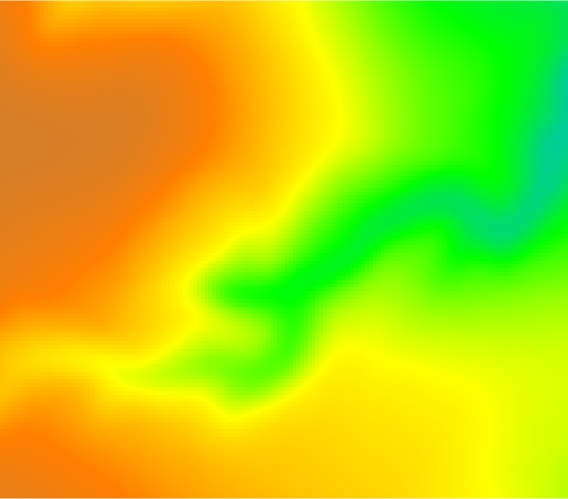
\includegraphics[width=\textwidth]{images/lrwoods_elevation.png}
%%[trim={0 0 0 1cm},clip,width=\textwidth]
%\label{fig_1_1}
%\textbf{a} \\
%\end{subfigure}
%%
%~ %add desired spacing between images, e. g. ~, \quad, \qquad, \hfill etc.
%%
%\begin{subfigure}[b]{0.3\textwidth}
%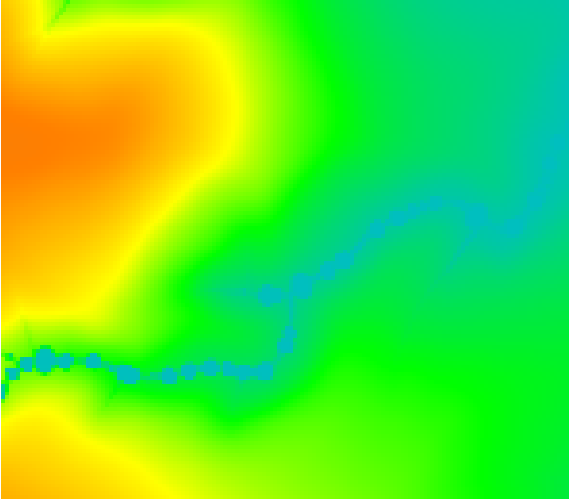
\includegraphics[width=\textwidth]{images/lrwoods_dynamics_flux_5m_30m.png}
%\label{fig_1_2}
%\textbf{b} \\
%\end{subfigure}
%%
%~ %add desired spacing between images, e. g. ~, \quad, \qquad, \hfill etc.
%%
%\begin{subfigure}[b]{0.3\textwidth}
%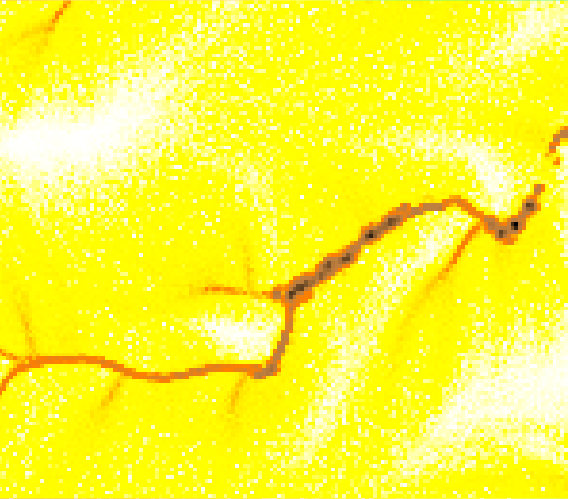
\includegraphics[width=\textwidth]{images/lrwoods_dynamics_erdep_5m_30m_flux.png} % REPLACE IMAGE
%\label{fig_1_3}
%\textbf{c} \\
%\end{subfigure}
%%
%\caption{{\bf Sediment flux based gully evolution.}
%\textbf{a)}
%A bare earth digital elevation model of gully in Lake Raleigh Woods, North Carolina derived from lidar data.
%\textbf{b)}
%The simulated evolution of the gully based on a detachment limited soil erosion regime.
%The landscape evolution model was run as a dynamic simulation with 155 mm/hr rainfall intensity for 5 minutes intervals over a 30 min period.
%This run of model carved deep pits along the center of the channel.
%\textbf{c)}
%Simulated sediment flux. 
%}
%\label{fig_1}
%\end{figure}
%
%\begin{figure}
%\centering
%%   
%\begin{subfigure}[b]{0.3\textwidth}
%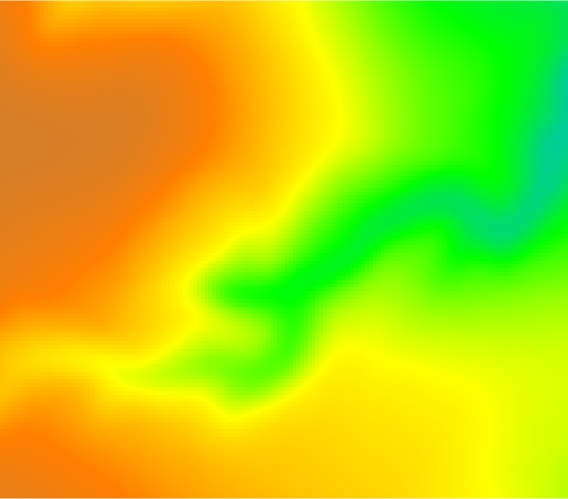
\includegraphics[width=\textwidth]{images/lrwoods_elevation.png}
%%[trim={0 0 0 1cm},clip,width=\textwidth]
%\label{fig_2_1}
%\textbf{a} \\
%\end{subfigure}
%%
%~ %add desired spacing between images, e. g. ~, \quad, \qquad, \hfill etc.
%%
%\begin{subfigure}[b]{0.3\textwidth}
%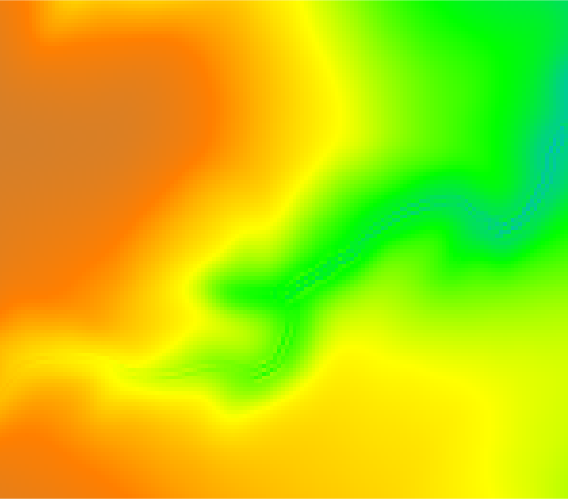
\includegraphics[width=\textwidth]{images/lrwoods_dynamics_erdep_5m_30m.png}
%\label{fig_2_2}
%\textbf{b} \\
%\end{subfigure}
%%
%~ %add desired spacing between images, e. g. ~, \quad, \qquad, \hfill etc.
%%
%\begin{subfigure}[b]{0.3\textwidth}
%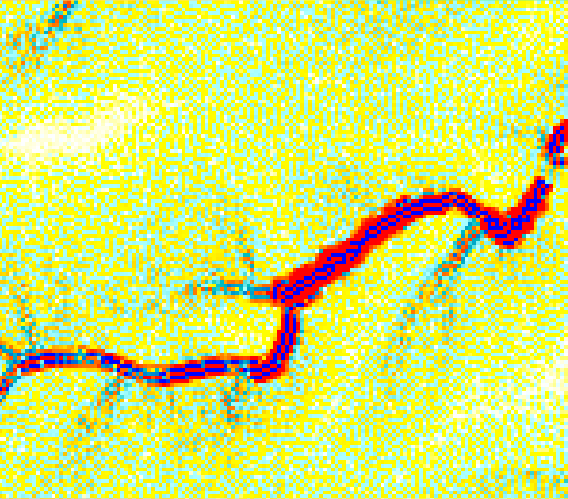
\includegraphics[width=\textwidth]{images/lrwoods_dynamics_erdep_5m_30m_erdep.png} % REPLACE IMAGE
%\label{fig_2_3}
%\textbf{c} \\
%\end{subfigure}
%%
%\caption{{\bf Erosion - deposition based gully evolution.}
%\textbf{a)}
%A bare earth digital elevation model of gully in Lake Raleigh Woods, North Carolina derived from lidar data.
%\textbf{b)}
%The simulated evolution of the gully based on a transport capacity limited  soil erosion regime.
%The landscape evolution model was run as a dynamic simulation with 155 mm/hr rainfall intensity for 5 minutes intervals over a 30 min period.
%This run of model carved a deeper channel, accumulated deposited sediment along the centerline of the channel, and accumulated deposited sediments along the banks of the channel.
%\textbf{c)}
%Simulated erosion-deposition. 
%}
%\label{fig_1}
%\end{figure}
%
%\begin{figure}
%\centering
%%   
%\begin{subfigure}[b]{0.4\textwidth}
%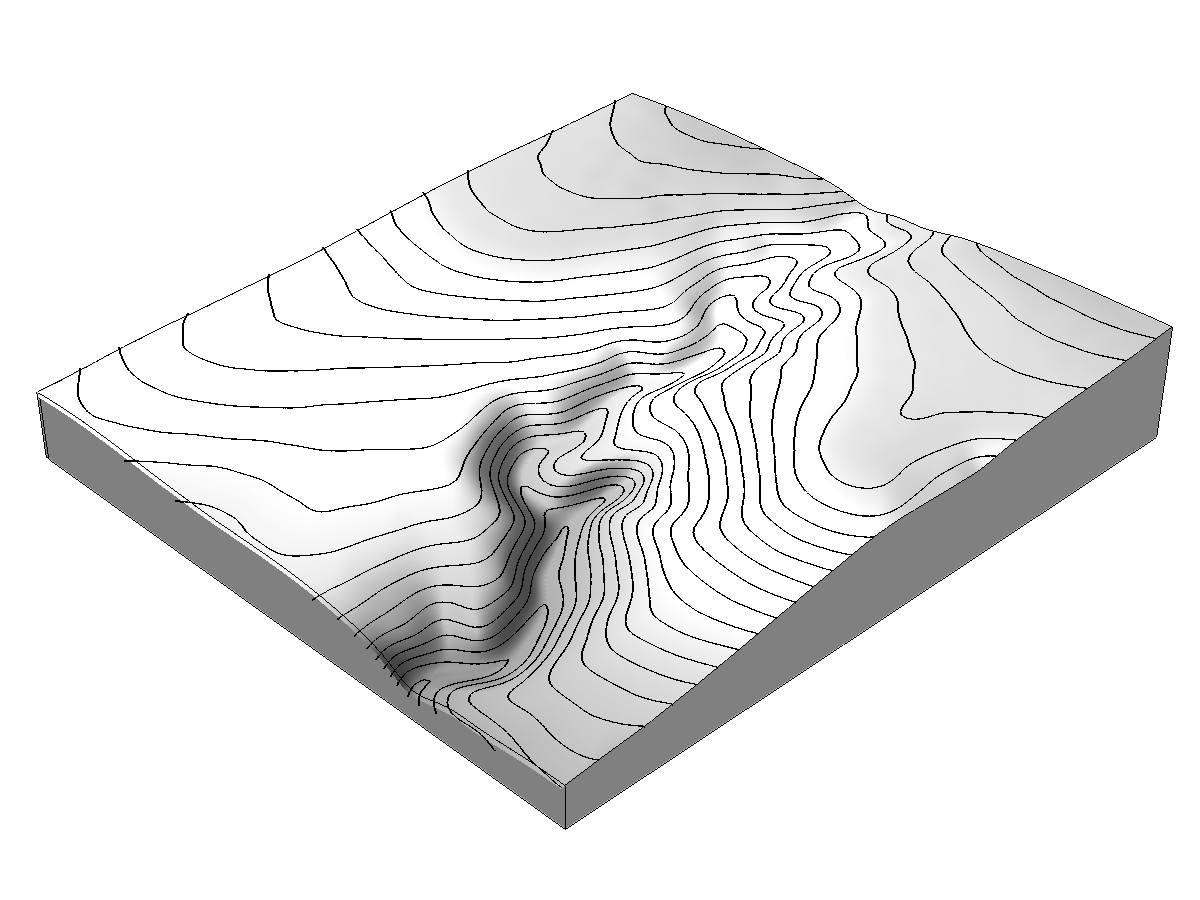
\includegraphics[width=\textwidth]{images/dem.png}
%%[trim={0 0 0 1cm},clip,width=\textwidth]
%\label{fig_2_1}
%\textbf{a} \\
%\end{subfigure}
%%
%~ %add desired spacing between images, e. g. ~, \quad, \qquad, \hfill etc.
%%
%\begin{subfigure}[b]{0.4\textwidth}
%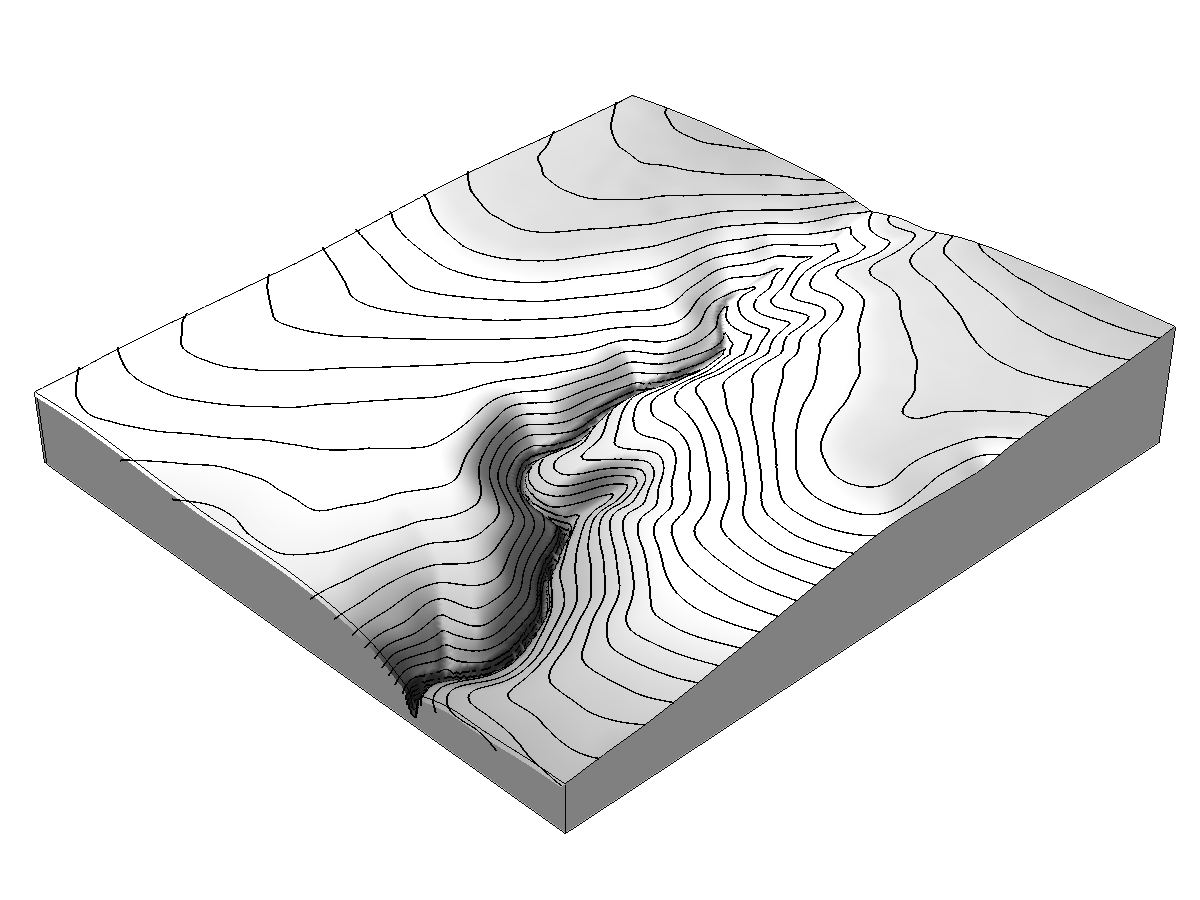
\includegraphics[width=\textwidth]{images/evolved_dem.png}
%\label{fig_2_2}
%\textbf{b} \\
%\end{subfigure}
%%
%\caption{{\bf Sediment flux based gully evolution.}
%\textbf{a)}
%A gully in Lake Raleigh Woods, North Carolina.
%\textbf{b)}
%The simulated evolution of the gully based on a detachment limited soil erosion regime. 
%The landscape evolution model was run as a steady state simulation with 155 mm/hr rainfall intensity for 10 minutes to model a 10-year storm event. 
%This run of the model carved a deep incision along the centerline of the channel.
%}
%\label{fig_2}
%\end{figure}
%
%\begin{figure}
%\centering
%%   
%\begin{subfigure}[b]{0.4\textwidth}
%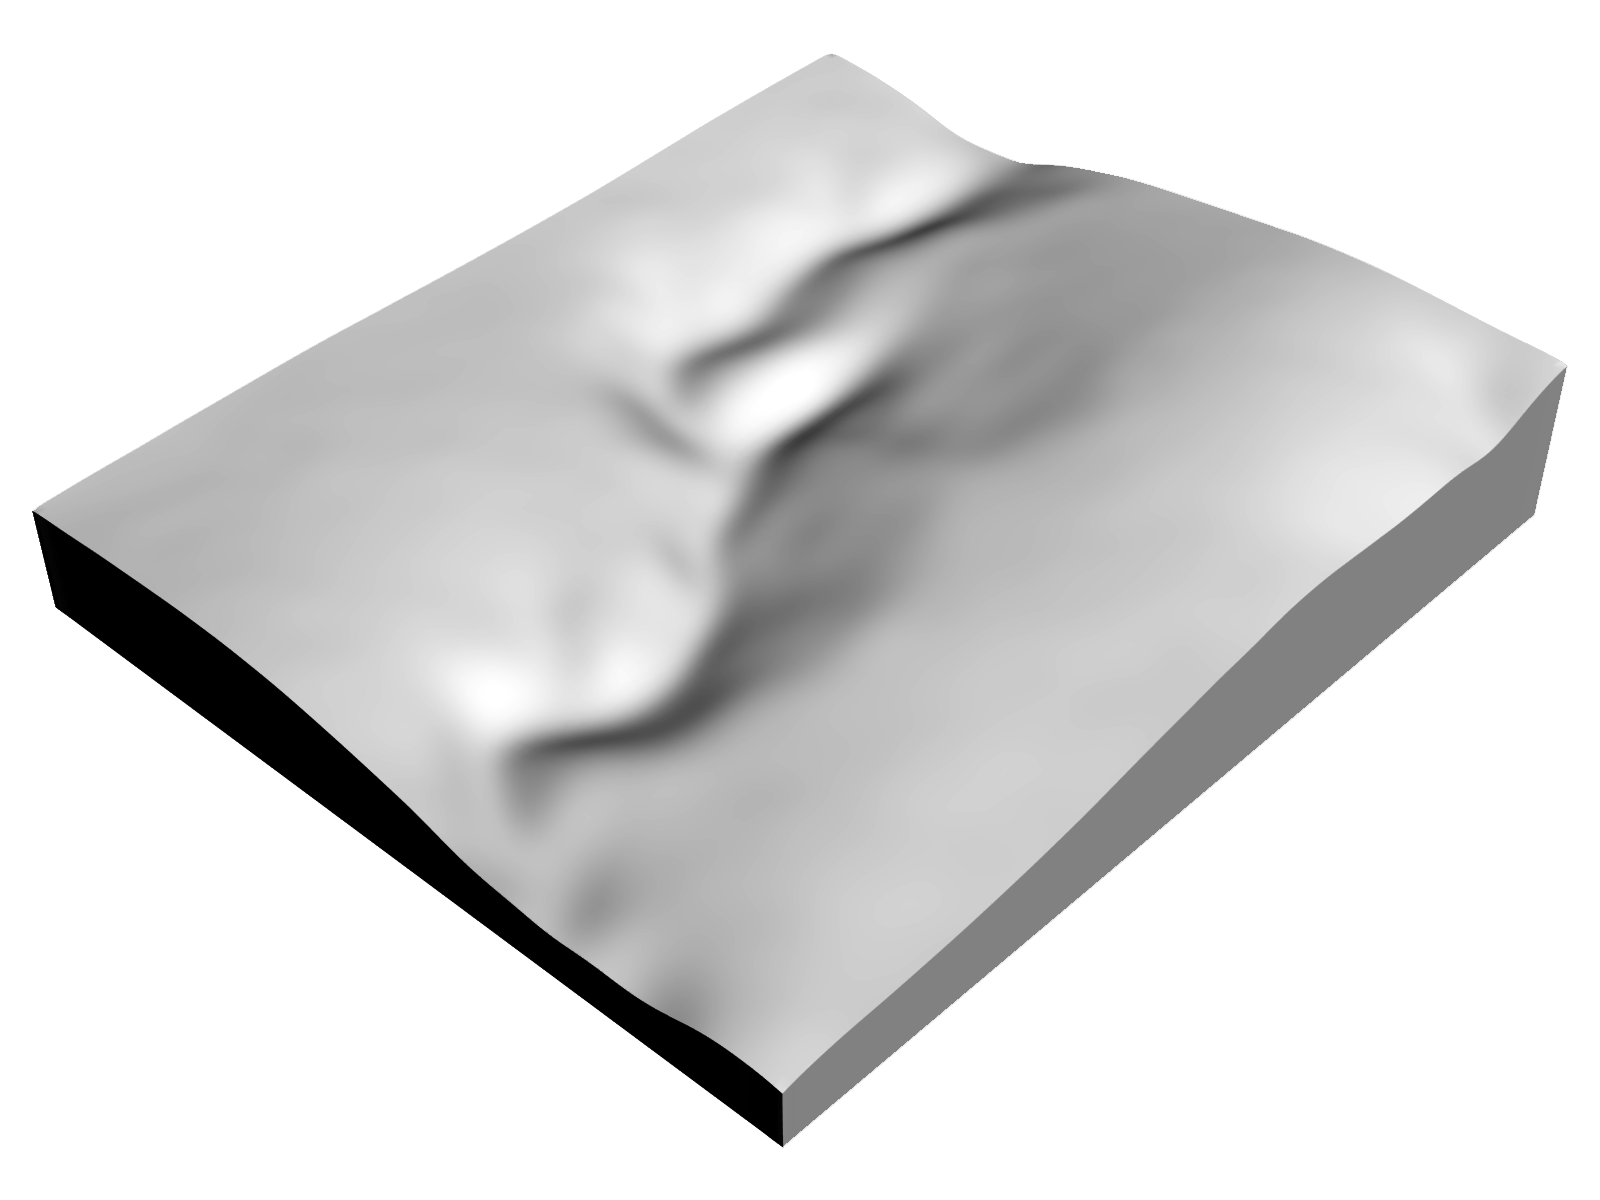
\includegraphics[width=\textwidth]{images/elevation_render.png}
%%[trim={0 0 0 1cm},clip,width=\textwidth]
%\label{fig_3_1}
%\textbf{a} \\
%\end{subfigure}
%%
%~ %add desired spacing between images, e. g. ~, \quad, \qquad, \hfill etc.
%%
%\begin{subfigure}[b]{0.4\textwidth}
%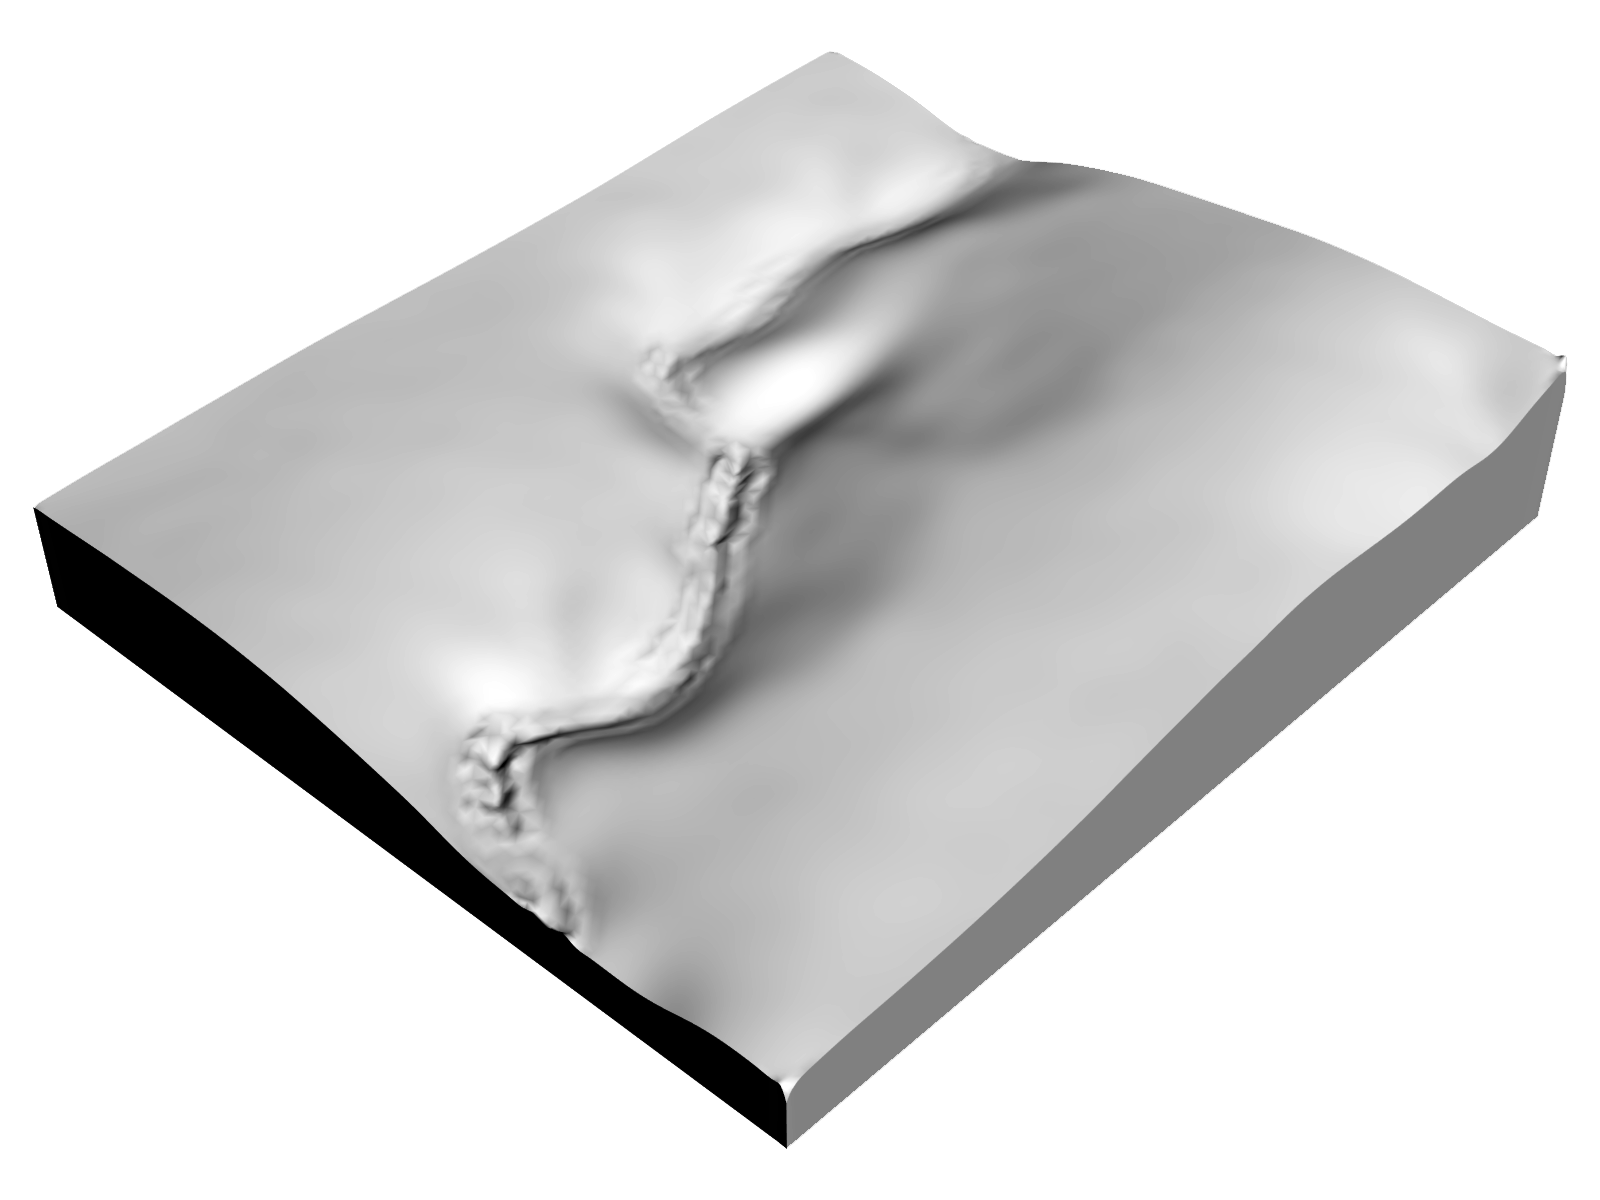
\includegraphics[width=\textwidth]{images/evolved_elevation_render.png}
%\label{fig_3_2}
%\textbf{b} \\
%\end{subfigure}
%%
%\caption{{\bf Erosion-deposition based gully evolution.}
%\textbf{a)}
%A gully in Lake Raleigh Woods, North Carolina.
%\textbf{b)}
%The simulated evolution of the gully based on a transport capacity limited  soil erosion regime.
%The landscape evolution model was run as a dynamic simulation with 155 mm/hr rainfall intensity for 5 minutes intervals over a 30 min period.
%This run of model carved a deeper channel, accumulated deposited sediment along the centerline of the channel, and accumulated deposited sediments along the banks of the channel.
%}
%\label{fig_3}
%\end{figure}

\clearpage
% -------------------------------- TANGIBLE --------------------------------
\section{Tangible landscape evolution}

Tangible Landscape -- a tangible user interface tightly integrated with a geographic information system for intuitively sketching in 3D \cite{petrasova2015}. Conceptually, Tangible Landscape couples a physical model with a digital model in a real-time feedback cycle of 3D scanning, geospatial modeling and simulation, and projection in order to physically manifest digital data as tangible bits. With tangible bits users can directly, physically feel and manipulate data with their bodies -- naturally, intuitively understanding space, form, and process. Tangible Landscape is available on Github at \url{https://github.com/ncsu-osgeorel/grass-tangible-landscape}.

%\paragraph{Testing}
We coupled Tangible Landscape with the landscape evolution model to test the model and experiment with strategies for restoration. 
We used Tangible Landscape to computationally steer the landscape evolution model and interactively explore the relationship between overland flow patterns and changes in topography. By manually changing the physical model of the landscape 
we change the topography used by the model.

\begin{figure*}
\centering
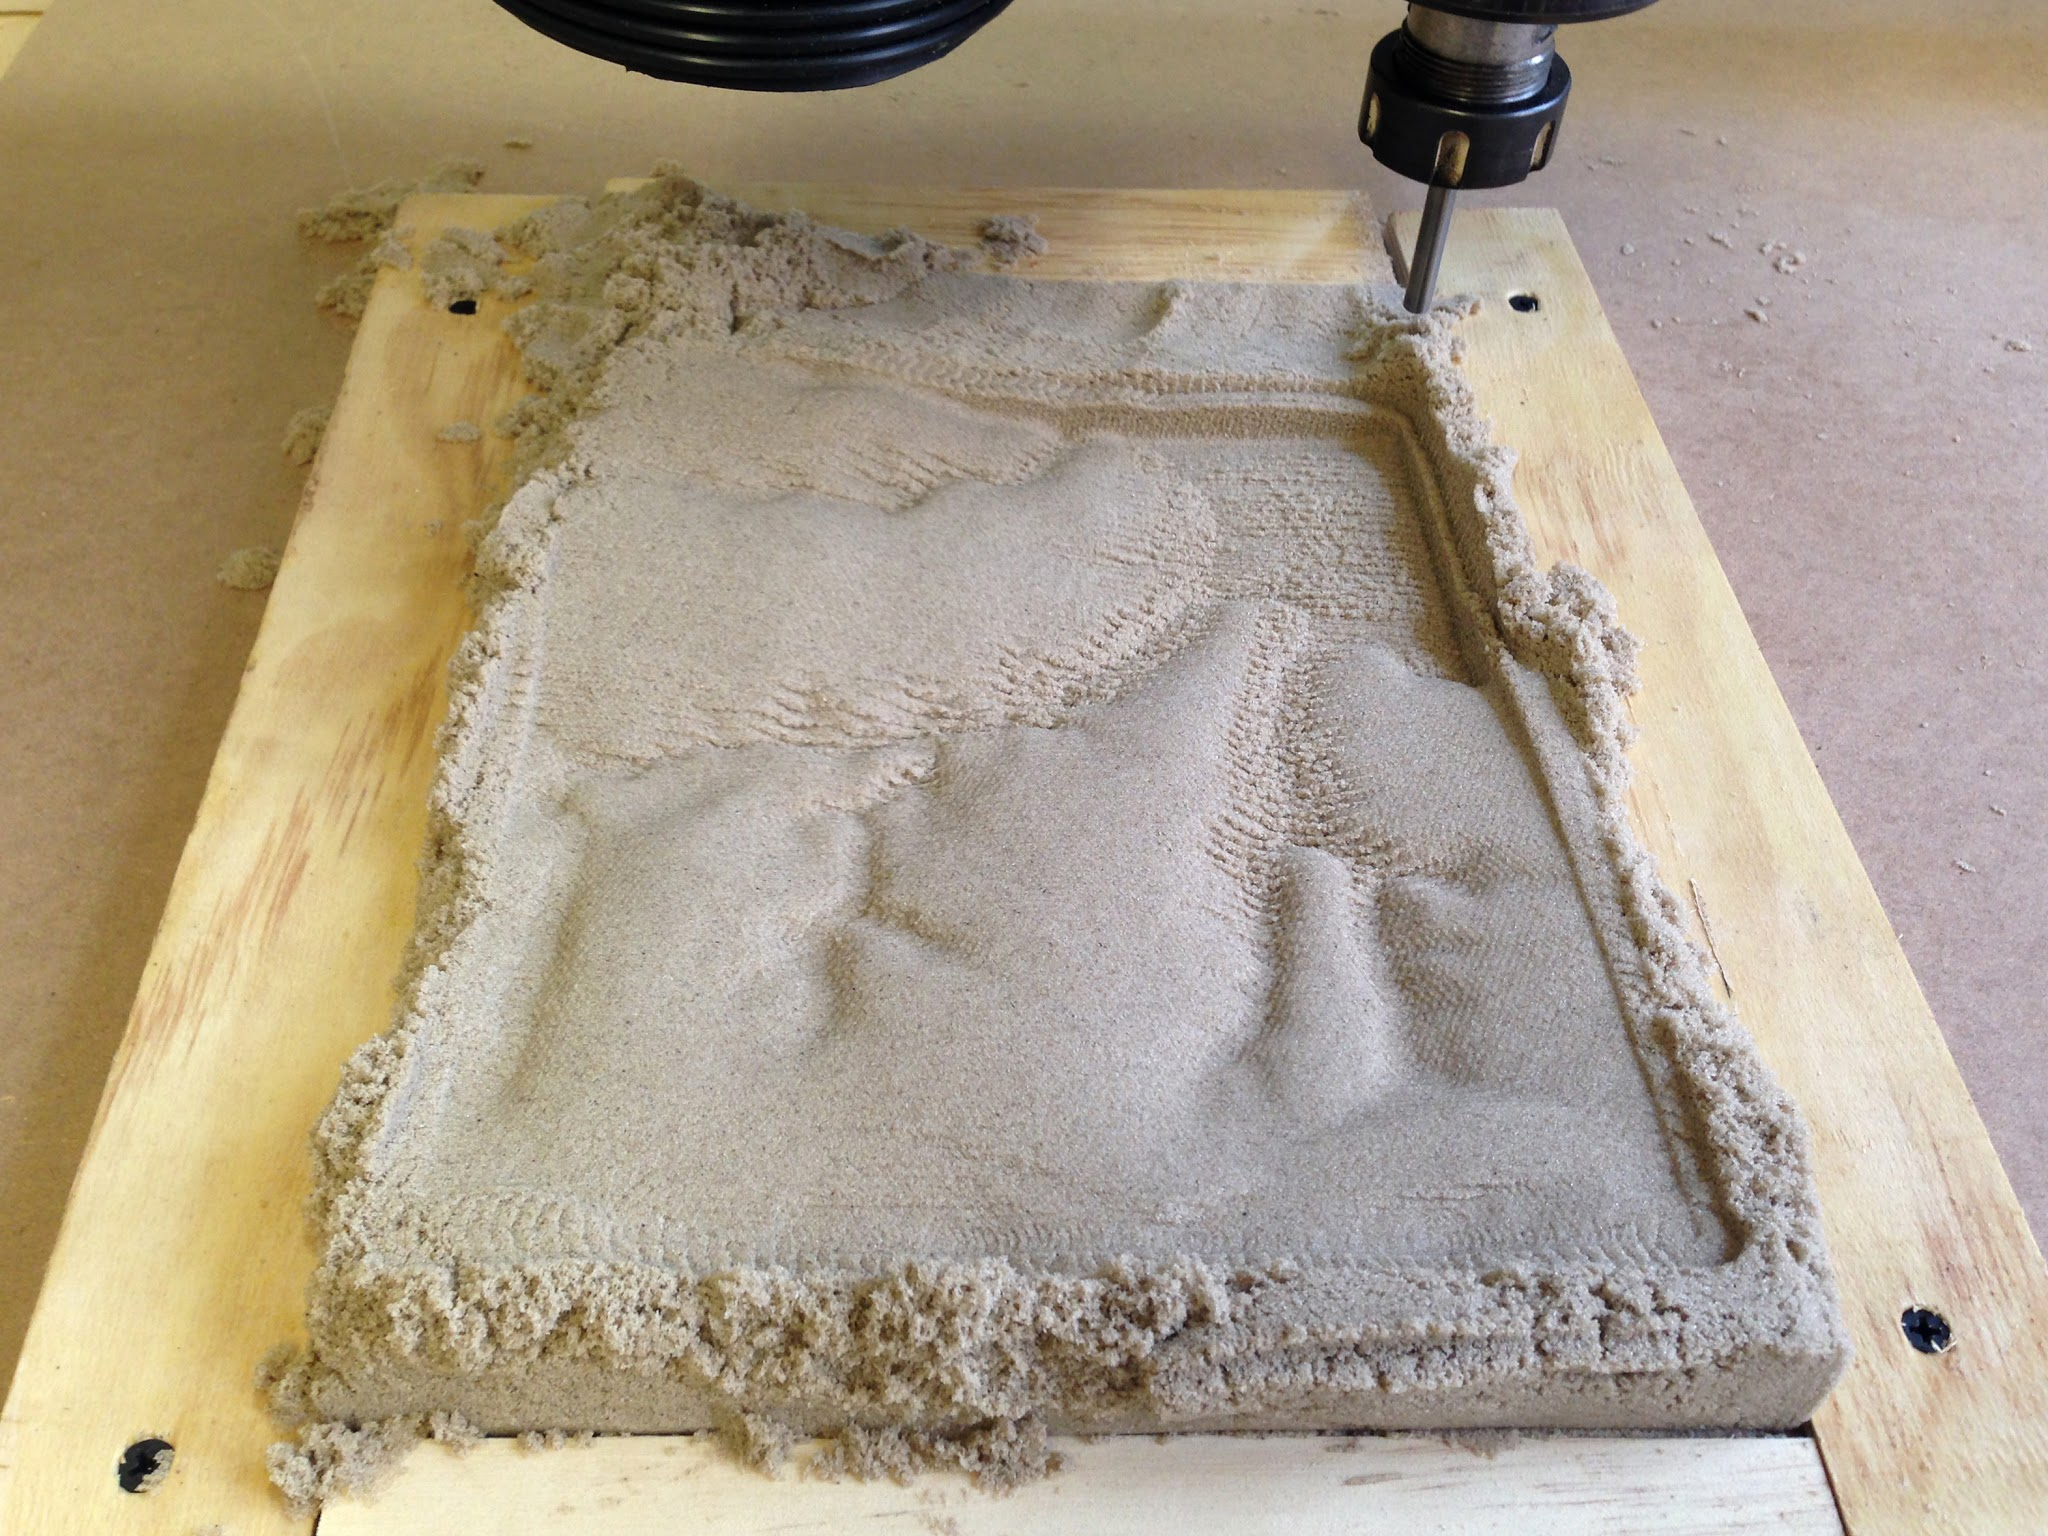
\includegraphics[width=\textwidth]{images/cnc_sand.jpg}
\caption{{\bf Rapid prototyping.}
3-axis CNC fabrication of the evolved landscape in polymer-enriched sand using a plunge cut.}
\label{fig:cnc_sand}
\end{figure*}

% -------------------------------- DISCUSSION --------------------------------
\section{Discussion}

\subsection{Future work}
\begin{enumerate}
\item Test the model on historical data
\item Test the model with UAS Sfm time-series
%\item Empirically calibrate the parameters
\item Implement as a Tangible Landscape analysis
\item Live, in-situ fabrication in polymer-enriched sand with a robotic arm
\end{enumerate}

\section{Conclusion}

% -------------------------------- APPENDIX --------------------------------
\appendix

\section{Supporting information}

\subsection{Code}\label{code}
{\bf Github repository}

\subsection{Data}\label{data}
{\bf GRASS GIS Mapset}

\subsection{3D models}\label{3d_models}
{\bf \ldots}

\subsection{Tangible Landscape}\label{tangible_landscape}
{\bf \ldots}

% -------------------------------- BIBLIOGRAPHY --------------------------------

% \bibliographystyle{elsarticle-num}
 \bibliographystyle{elsarticle-harv}
% \bibliographystyle{elsarticle-num-names}
% \bibliographystyle{model1a-num-names}
% \bibliographystyle{model1b-num-names}
% \bibliographystyle{model1c-num-names}
% \bibliographystyle{model1-num-names}
% \bibliographystyle{model2-names}
% \bibliographystyle{model3a-num-names}
% \bibliographystyle{model3-num-names}
% \bibliographystyle{model4-names}
% \bibliographystyle{model5-names}
% \bibliographystyle{model6-num-names}

\bibliography{landscape_evolution.bib}


\end{document}

